%%%%%%% NOTE %%%%%%%
% Typeset thrice to get positioning
%%%%%%%%%%%%%%%%%%

\documentclass{article}
\usepackage{tikz, graphicx}

%% USER DEFINED %%
\def\streetx{536}
\def\streety{247}
%%%%%%%%%%%%%

\begin{document}
\thispagestyle{empty}
\tikzset{every picture/.append style={xscale=1/sqrt(2)}}
\newcommand\mytikz[2]{
  \begin{tikzpicture}
    [overlay, remember picture, xscale=sqrt(2)]
    \draw (current page.center) ++(#1)
    node {\begin{tikzpicture}#2\end{tikzpicture}};
    \end{tikzpicture}
  }
\pgfmathtruncatemacro\xnext{\streetx+2}
\pgfmathtruncatemacro\ynext{\streety+2}
\pgfmathtruncatemacro\xa{\streetx/100}
\pgfmathtruncatemacro\ya{\streety/100}
\pgfmathtruncatemacro\xb{(\streetx-\xa*100)/10}
\pgfmathtruncatemacro\yb{(\streety-\ya*100)/10}
\pgfmathtruncatemacro\xc{\streetx-\xa*100-\xb*10}
\pgfmathtruncatemacro\yc{\streety-\ya*100-\yb*10}
%\xa,\xb,\xc;
%\ya,\yb,\yc;
\mytikz{0,11in/4}{
\mytikz{0,11in/4}{
  \node {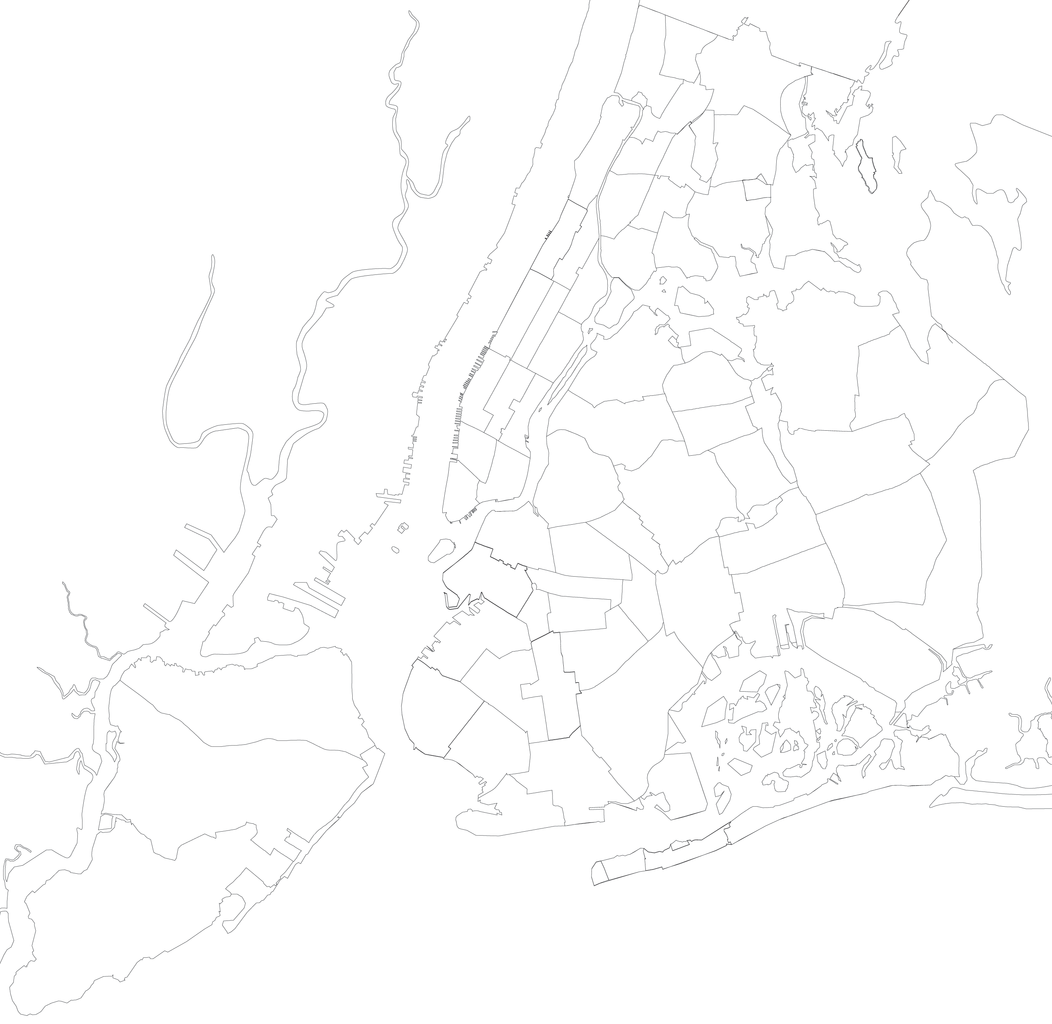
\includegraphics[scale=0.3]{pattern-streets2.png}};
  }
  [scale=0.95]
  \draw[blue, line width=1mm] (\xa,\ya) rectangle ++ (1,1);
  \draw (\xa,\ya) coordinate (a1) 
    ++(right:1) coordinate (a2)
    ++(up:1) coordinate (a3)
    ++(left:1) coordinate (a4)
    ;
  \draw[step=0.1] (\xa,\ya) grid ++ (1,1);
  \draw[step=0.02] (\xa+\xb/10,\ya+\yb/10) grid ++ (0.1,0.1);
  \fill[red](\xa+\xb/10+\xc/100,\ya+\yb/10+\yc/100-1/100) rectangle ++ (0.02,0.02);
  \draw (-0.5,-0.5) grid (20.5,10.5);
  \draw (0,-0.5) node [left, rotate=90] {Avenue 0};
  \draw (0,10.5) node [right, rotate=90] {\phantom{Avenue 0}};
  \foreach \x in {1,...,20}{
    \draw (\x,-0.5) node [left, rotate=90] {\x00};
    }
  \draw (-0.5,0) node [left] {Avenue 1};
  \draw (20.5,0) node [right] {\phantom{Avenue 1}};
  \foreach \x in {1,...,10}{
    \draw (-0.5,\x) node [left] {\x01};
    }
  }
\mytikz{-8.5in/4,-11in/4}{
  [scale=0.95]
  \draw[blue, line width=2mm]  (0,0) rectangle (10,10);
  \draw (0,0) coordinate (b1) 
    ++(right:10) coordinate (b2)
    ++(up:10) coordinate (b3)
    ++(left:10) coordinate (b4)
    ;
  \draw[red, line width=0.5mm] 
    (\xb+\xc/10, \yb+\yc/10-0.1) rectangle ++ (2mm,2mm);
  \draw
    (\xb+\xc/10, \yb+\yc/10-0.1) coordinate (c1)
    ++(right:2mm) coordinate (c2)
    ++(up:2mm) coordinate (c3)
    ++(left:2mm) coordinate (c4)
    ;
  \draw[step=2mm] (\xb,\yb) grid ++ (1,1);
  \foreach \x/\y in {2/3, 4/5, 6/7, 8/9}{
    \begin{scope}
      [inner sep=0.75mm, every node/.style={scale=0.35}]
      \draw (\xb+\x/10,\yb) 
        node [left, rotate=90] {Ave \xa\xb\x};
      \draw (\xb,\yb+\y/10-0.1)
        node [left] {Ave \ya\yb\y};
      \end{scope}
    }
  \draw (-0.5,-0.5) grid (10.5,10.5);
  \draw (0,-0.5) node [left, rotate=90] {Avenue \xa00};
  \draw (-0.5,0) node [left] {Avenue \ya01};
  \foreach \x in {1,...,10}{
    \pgfmathtruncatemacro\xax{\xa*10+\x}
    \pgfmathtruncatemacro\yax{\ya*10+\x}
    \draw (\x,-0.5) node [left, rotate=90] {\xax0};
    \draw (-0.5,\x) node [left] {\yax1};
    }
  }
\mytikz{8.5in/4,-11in/4}{
  [scale=0.7]
  \draw[red, line width=2mm]  (0,0) rectangle (10,10);
  \draw (0,0) coordinate (d1)
    ++(right:10) coordinate (d2)
    ++(up:10) coordinate (d3)
    ++(left:10) coordinate (d4)
    ;
  \draw (0,0) rectangle (10,10);
  \clip (0-1.4*3,0-3) rectangle (10+1.4*3,10+3);
  \draw (0-1.4*4,0) rectangle (-1.4*2,10);
  \draw (10+1.4*2,0) rectangle (10+1.4*4,10);
  \draw (0,0-4) rectangle (10,0-2);
  \draw (0,10+4) rectangle (10,10+2);
  \begin{scope}[every node/.style={scale=1.5}]
    \draw (0-1.4,5) node [rotate=90] {Avenue \streetx};
    \draw (10+1.4,5) node [rotate=90] {Avenue \xnext};
    \draw (5,0-1) node {Avenue \streety};
    \draw (5,10+1) node {Avenue \ynext};
    \end{scope}
  \foreach \x in {0,...,49}{
    \pgfmathtruncatemacro\bot{100*\xc+2*\x+1}
    \pgfmathtruncatemacro\left{100*\yc+2*\x+1}
    \pgfmathtruncatemacro\top{100*\xc+2*\x}
    \pgfmathtruncatemacro\right{100*\yc+2*\x}
    \begin{scope}[every node/.style={scale=0.4}]
      \draw (\x/5+0.1,0) node [left, rotate=90] {\xa\xb\bot};
      \draw (\x/5+0.1,0-2) node [right, rotate=90] {\xa\xb\top};
      \draw (0,\x/5+0.1) node [left] {\ya\yb\left};
      \draw (0-1.4*2,\x/5+0.1) node [right] {\ya\yb\right};
      \draw (\x/5+0.1,10) node [right, rotate=90] {\xa\xb\top};
      \draw (\x/5+0.1,10+2) node [left, rotate=90] {\xa\xb\bot};
      \draw (10,\x/5+0.1) node [right] {\ya\yb\right};
      \draw (10+1.4*2,\x/5+0.1) node [left] {\ya\yb\left};
      \end{scope}
    }
  }
\begin{tikzpicture}
  [overlay, remember picture]
  \draw[blue]
    (a1) -- (b1)
    (a2) -- (b2)
    (a3) -- (b3)
    (a4) -- (b4)
    ;
  \draw[red]
    (c1) -- (d1)
    (c2) -- (d2)
    (c3) -- (d3)
    (c4) -- (d4)
    ;
  \end{tikzpicture}
\end{document}  